\documentclass[pdf,aspectratio=169]{beamer}
\usepackage[]{hyperref,graphicx,siunitx,booktabs,lmodern}
\usepackage{physics}
\usepackage{em-commands}
\mode<presentation>{\usetheme{EM}}

%Question Numbering
\newcounter{questionnumber}
\newcommand{\qnum}{%
	\stepcounter{questionnumber}%
	Q\arabic{questionnumber}
}
\resetcounteronoverlays{questionnumber}

\graphicspath{ {../Images/} }

\sisetup{per-mode=symbol}

\tikzstyle{plate}=[draw, very thick, minimum width=4cm, minimum height=1cm, fill=gray!40, anchor=south]

%preamble
\title{Hysterical over Hysteresis}
\date{November 26, 2018}
\author{Jed Rembold}

\begin{document}
\renewcommand{\theenumi}{\Alph{enumi}}

\begin{frame}{Announcements}
	\begin{itemize}
		\item Homework
			\begin{itemize}
				\item Homework 11 due Wednesday night
				\item Number 4 is a sweet problem but a bit of a doozy, so don't leave everything until last minute
			\end{itemize}
		\item Still working on grading the take-home portion of the test, we'll talk the in-class portion through though today
		\item Did you record yourself explaining an E\&M concept to a clueless family member but forget to send it to me? Get it sent!
	\end{itemize}
\end{frame}

\begin{frame}{Test Discussion: 1}
		Given the current distribution below, what would be the total value of the magnetic field integrated along the path indicated in the direction of the arrows?
		\begin{center}
			\tdplotsetmaincoords{70}{110}
			\begin{tikzpicture}[use Hobby shortcut, tdplot_main_coords, scale=1.3]
				\tdplotsetcoord{p1}{3}{45}{90}
				\tdplotsetcoord{p2}{2}{45}{90}
				\tdplotsetcoord{p3}{4}{45}{-90}
				\draw[-latex, ultra thick] (p1xy) -- +(0,0,-2) node[right,math] {\cur_1};
				\draw[ultra thick] (p2xy) to[bend left] +(0,-1,-2);
				\draw[ultra thick, -latex] (p3xy) -- +(0,1,-2) node[below,math] {\cur_3};
				\draw[fill=white, thick, closed, ->>-=0.1 to 1 by 0.1, xyplane=0, name path=c] (0,-1) .. (-2,-1) .. (-3,-2) .. (-4,-1) .. (-3,2) .. (-2,2) .. (-1,1) .. (2,2) .. (2,-2);
				\draw[ultra thick] (p1) -- (p1xy);
				\draw[ultra thick, -latex] (p2xy) to[bend right] +(0,-1,2) node[above,math] {\cur_2};
				\draw[ultra thick] (p3xy) -- +(0,-1,2);

				\draw[dashed] (p1xy) --+(0,1,0) coordinate[pos=0.25] (a1)
					(p2xy) --+(0,-1,0) coordinate[pos=0.25] (a2)
					(p3xy) --+(0,-1,0) coordinate[pos=0.25] (a3);
				\draw (p1xy)++(0,0,.25)--++(0,.25,0)--++(0,0,-.25)
					(p2xy)++(0,0,.25)--++(0,-.25,0)--++(0,0,-.25);
					%($(p3xy)!.25cm!(p3)$) to[bend right] (a3); 
				\tdplotsetthetaplanecoords{-90}
				\tdplotdrawarc[tdplot_rotated_coords]{(p3xy)}{0.25}{90}{35}{anchor=south east}{$\alpha$}
			\end{tikzpicture}
		\end{center}
\end{frame}

\begin{frame}{Test Discussion: 2}
	\begin{columns}
		\column{0.5\textwidth}
		An electron enters the below region traveling at \SI{500}{\m\per\s} to the right. If both the $\ef$ and $\mf$ have a magnitude of \num{1e-6} \si{\volt\per\meter} or \si{\tesla} respectively, what trajectory best describes the resulting path of the particle? The electric field is pointing upward and the magnetic field is pointing out of the page. (You can assume the same magnetic and electric fields extend everywhere in the region.)
		
		\column{0.5\textwidth}
		\begin{center}
			\begin{tikzpicture}
				\foreach \x in {1,2,...,4}{
					\draw[thick, -latex] (\x,-2) -- (\x,3);
					\foreach \y in {-1.5,-.5,...,1.5} \node[font=\Large] at (\x+.5,\y) {$\odot$};
				}
				\node[point, label={above:e$^-$}] (e) at (-1,0) {};
				\draw[-latex, very thick] (e) --+(1,0) coordinate[right] (s);
				\node[above] at (3,3) {$\ef$};
				\node[below] at (2.5,-1.7) {$\mf$};

				\draw[ultra thick] (s) .. controls +(0:3) and +(135:1) .. (5,-2) node[right, font=\LARGE] {A};
				\draw[ultra thick] (s) -- (5,0) node[right, font=\LARGE] {B};
				\draw[ultra thick] (s) .. controls +(0:3) and +(-135:1) .. (5,2) node[right, font=\LARGE] {C};
				\draw[ultra thick] (s) arc (-90:90:2cm) node[left, font=\LARGE] {D};
			\end{tikzpicture}
		\end{center}
	\end{columns}
\end{frame}

\begin{frame}{Test Discussion: 3}
		A cylinder whose axis points along the $\zhat$ direction has a baked-in polarization of 
		\[\pol = P_0 (\vu{s} + s \vu*{\phi})\]
		where $s$ is the cylindrical coordinate and $P_0$ is a constant. Determine where any bound charge might exist on the surface or in the bulk and calculate any corresponding charge densities.
		\begin{flushleft}
			\begin{tikzpicture}
				\pic at (0,0) {cyl=white/.75/3/4};
				\draw[very thick, -latex] (0,0) -- +(0,.5) node[above]{$\zhat$};
			\end{tikzpicture}
		\end{flushleft}
\end{frame}

\begin{frame}{Test Discussion: 4}
		A gas is comprised of the below neutral molecule. When the gas is placed in a region with a strong electric field, will the net electric field in the gas will be greater, smaller, or about the same as the original external field? Explain yourself for full points.
		\begin{flushright}
			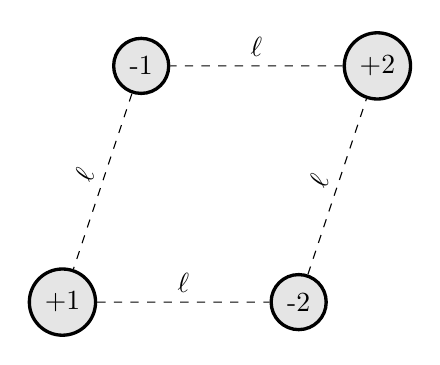
\begin{tikzpicture}
				\node[circle, draw, very thick, fill=gray!20] (p1) at (0,0) {+1};
				\node[circle, draw, very thick, fill=gray!20] (p2) at (4,3) {+2};
				\node[circle, draw, very thick, fill=gray!20] (p3) at (3,0) {-2};
				\node[circle, draw, very thick, fill=gray!20] (p4) at (1,3) {-1};
				\draw[dashed] (p1) -- (p3) node[midway,sloped,above]{$\ell$} -- (p2) node[midway,sloped,above]{$\ell$} -- (p4) node[midway,sloped,above]{$\ell$} -- (p1) node[midway,sloped,above]{$\ell$};
			\end{tikzpicture}	
		\end{flushright}
\end{frame}

\begin{frame}{Test Discussion: 5}
		An infinitely long cylinder with radius $R$ is oriented in the $\zhat$ direction and has a volume current density of 
		\[\vcd = J_0 s \vu*{\phi}\]
		where $s$ is the cylindrical coordinate and $J_0$ is a constant. Determine the magnetic field $\mf$ everywhere.
\end{frame}

\begin{frame}{Test Discussion: 6}
	A record with radius of \SI{15}{\centi\meter} has \SI{500}{\milli\coulomb} of charge evenly spread over its circular surface. The record is spinning at a rate of 1 revolution every second. What is the magnitude and direction of the magnetic field at the center of the record?
\end{frame}


\section{Resuming our regularly scheduled playback\ldots}


\begin{frame}{\qnum}
	\begin{columns}
		\column{0.5\textwidth}
		\begin{center}
			\begin{tikzpicture}
				\draw[very thick, fill=violet!20, name path=cv]
					(-3,-3) .. controls +(0:5) and +(180:2) .. (3,3)
					.. controls +(180:5) and +(0:2) .. (-3,-3);
				\path[thick, -latex] 
					(-3,0) edge node[at end,right,math] {H} (3,0)
					(0,-3) edge node[at end,above,math] {B} (0,3);
				\path[name path=y] (0,-3) -- (0,3);
				\node[name intersections={of=cv and y, by=p}, point] at (p) {};
			\end{tikzpicture}
		\end{center}
		
		\column{0.5\textwidth}
		Given the hysteresis curve to the left, what can be stated about the indicated point?
		\begin{enumerate}
			\item No magnetic field is being applied to the ferromagnet
			\item The ferromagnet currently has 0 permanent magnetization
			\item Increasing the applied magnetic field will increase the magnitude of the ferromagnet's magnetic field
			\item A negative magnetic field is being applied to the ferromagnet
		\end{enumerate}
		
	\end{columns}
\end{frame}

\begin{frame}{\qnum}
	What are the units for the area under a $\af$-$\mf$ hysteresis curve?
	\begin{enumerate}
		\item $\displaystyle\si[per-mode=fraction]{\square\tesla \ampere\per\newton}$
		\item $\displaystyle\si[per-mode=fraction]{\newton\per\square\meter}$
		\item $\displaystyle\si[per-mode=fraction]{\square\tesla}$
		\item $\displaystyle\si[per-mode=fraction]{\tesla\ampere\per\square\newton}$
	\end{enumerate}
\end{frame}







\end{document}
